\section*{Introduction}
EASIER and GIGADuck are two versions  of a radio detector tuned in the
C-band and  installed on Auger SD  station. They share  the same basic
design: the  sensor is a feed horn  antenna and it is  connected to an
amplifier.  The  Radio Frequency  (RF) signal is  then fed to  a power
detector which outputs a voltage  proportiobal to the logarithm of the
signal envelope. This  voltage is in turn adapted to  the SD front end
input and  is recorded as one of  the 6 FE input  channel (it replaces
one of the PMT anode signal).  EASIER was the original design, it uses
commercial TV antenna  pointing toward the zenith~\cite{gapeasier} and
is  implemented on  47 stations,  while GIGADuck  is installed  on one
hexagon  and has  the six  surrounding detector  pointing at  a zenith
angle of 20 degree and  an azimuth of the central detector\cite{gapGD}
direction.\\For such  detector, a figure  of merit of  the sensitivity
can be written as:
\begin{equation}
  F = \frac{k_{B}T_{sys}}{A_{eff}\sqrt{\Delta t}{\Delta \nu}}
\end{equation}
where $\rm  k_{B}$ is  the Boltzmann constant,  $\rm T_{sys}$  is the
system noise temperature,  $\rm A_{eff}$ is the effective  area of the
antenna, and $\rm \sqrt{\Delta t}{\Delta \nu}$ is the number of sample
on  can integrate  on with  $\rm \Delta  \nu$ the  bandwidth  and $\rm
\Delta  t$ the  length  of  the expected  signal.\\  The system  noise
temperature  is thus a  key parameter  in the  calibration of  a radio
detector. For EASIER and GIGADuck  detectors, the noise comes from the
thermal  noise  collected by  the  antenna,  $\rm  T_{ant} $  and  the
amplifier noise $\rm  T_{elec}$. The noise added by  the element after
the amplifier are  reduced by the gain of  the amplifier, around 60dB,
and  is  thus negligible.   The  antenna  temperature  is obtained  by
integrating   the   sky  and   ground   temperature  (the   brightness
temperature) over 4$\rm \pi$ weighted by the antenna gain:
\begin{equation}
  T_{ant} = \int_{\theta =  0}^{\theta = \pi}\int_{\phi = 0}^{\phi =
    2\pi} T_{B} G(\theta,\phi) d\theta d\phi
\label{eq:tant}
\end{equation}
To measure the  electronic temperature, one has to  compare the output
power when the system is  irradiated with two known microwave sources.
One    reference   is    the   antenna    temperature    computed   in
equation~\ref{eq:tant}. The  second reference can be the  sun flux, it
is    used   for    the    GIGADuck   detector    and   detailed    in
section~\ref{sec:gigaduck}, however due to  a smaller antenna gain, we
can't  use  the  sun  signal  for  EASIER, we  then  use  the  antenna
temperature when the antenna points  toward the ground, this method is
detailed in~\ref{sec:easier}.


\section{Expected signal from the sun flux}
\label{sec:expectedsignal}
We present in this section the calculation of the expected signal from
the solar flux. The main ingredients are:
\begin{itemize}
\item the sun flux (the sun flux varies with time)
\item the sun path with respect to the antenna depending on the time of the year
\item the antenna pattern
\end{itemize}
Given these ingredients  one can estimate the additional  power at the
sun passage:
\begin{equation}
  P_{sun}(t) = \frac{1}{2}F_{sun}A_{eff}(\theta(t),\phi(t)) [W/Hz]
\end{equation}
where the  factor $\frac{1}{2}$ comes from  the polarization selection
of the antenna. 

\subsection{Sun flux}
The  sun  flux  is  measured  by dedicated  observatories  around  the
world\cite{nobeyama,canadianobs}  at several  frequencies. We  use the
flux at 2.8GHz  (so called F107) whis is widely  measured. In order to
extrapolate  to  the  frequency  band  we  are  interested  we  use  a
paramterization. In  the microwave frequency  range, the sun  flux has
two  main contributions~\cite{solarflux}:  a quiet  sun  component (or
background  component)  with  a  constant intensity  and  a  frequency
dependence as:
\begin{equation} 
 Sq \  [SFU] =  26.4 +  12.4 \ \nu  + 1.11\  \nu^2 \\ \rm  for \  (1 <
 \nu(GHz) < 20)
\end{equation}
a    second    contribution,   the    so    called   slowly    varying
component, its spectrum is parameterised as:
\begin{equation}
    Sv  \ [SFU]= \frac{0.64 ( F10.7 - 70 ) f^{0.4}}{ 1 + 1.56 ( ln \ ( \ f  \ / \  2.9 ) )^2}
\end{equation}
These spectra are shown in the figure~\ref{fig:spectra}
\begin{figure}[!ht]
  \centering
  \hspace*{-3ex}
  \subfigure{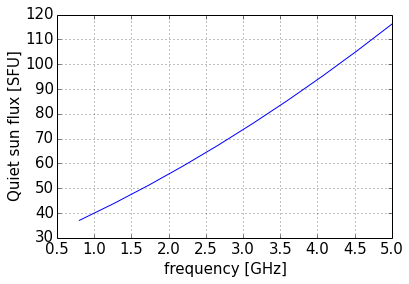
\includegraphics[width=0.49\linewidth]{quietsunspec.png}}
  \subfigure{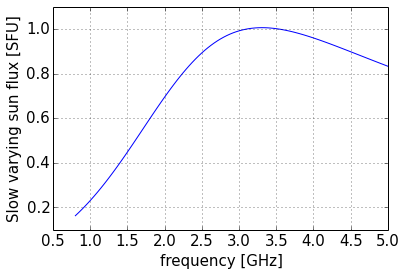
\includegraphics[width=0.49\linewidth]{varyingsunspec.png}}
  \caption{Left: quiet sun spectrum, Right: varying component spectrum}
  \label{fig:spectra}
\end{figure}
An   example  of   the   sun  flux   at   10.7cm  is   shown  in   the
Figure~\ref{fig:f107}. One  can notice  the quasi monthly  modulation that
can  be of  the  order  of 30-40\%  and  justify the  use  of a  daily
measurement instead of a month or a year average.
\begin{figure}[!ht]
  \centering
  \hspace*{-3ex}
  \subfigure{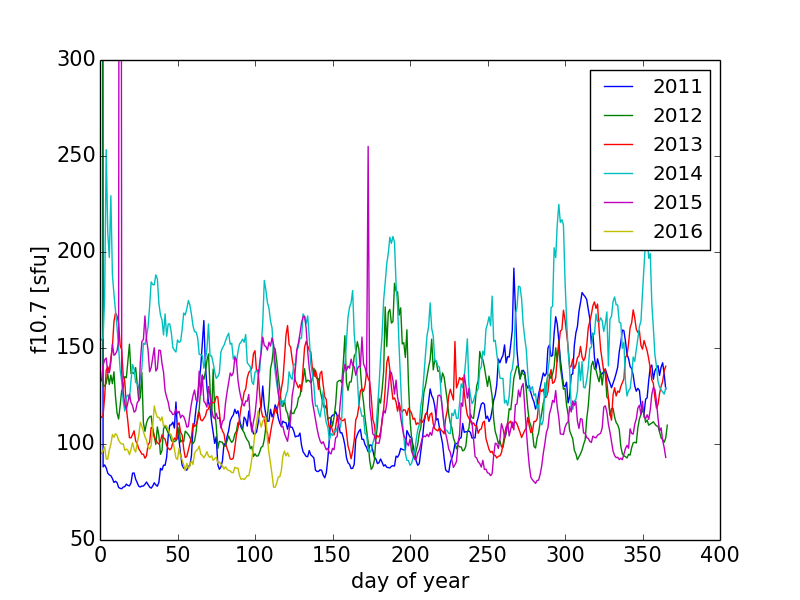
\includegraphics[width=0.49\linewidth]{f10_72011_2016.png}}
  \subfigure{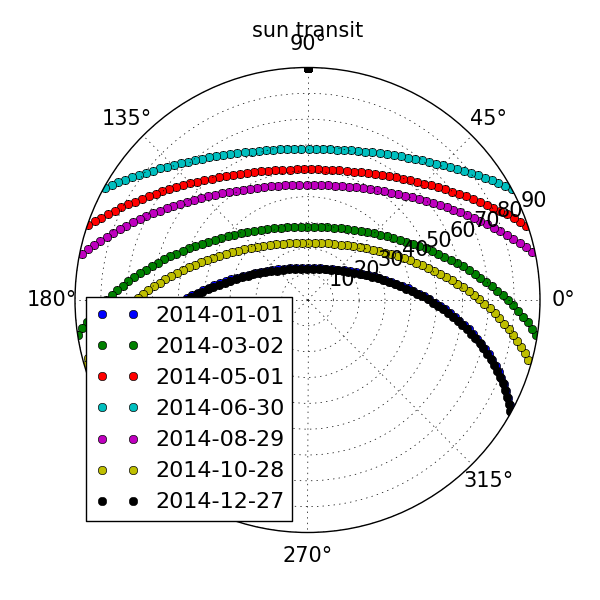
\includegraphics[width=0.49\linewidth]{sunpath.png}}
  \caption{Left: f107 from 2011 to  2015. Right: sun transit along the
    year}
  \label{fig:f107}
\end{figure}
\subsection{the sun transit}
The  other ingredient, the  sun transit  on the  sky of  Malarg\"ue is
found using the code Sun Position Algorithm (SPA)~\cite{spa}. Examples
of the  path during the year  are shown in polar  coordinate where the
radius is the zenith angle and  the angle is the azimuth (90 degree is
the north).
\subsection{the antenna pattern}
The  last ingredient  is  the effective  area  of the  antenna in  the
direction of the sun position.   The angular gain, directly related to
the effective  area, was measured  in anechoic chamber for  the EASIER
antennas~\cite{rapportdemesurechambreanechoic},   for   the   GIGADuck
detectors we rely on  pattern simulation performed with HFSS software.
Note that the antenna geometry is rather simple (horn antenna) so that
the simulations for our purpose  is reliable. The gain explored for an
EASIER  or a  GIGADuck  antenna (the  vertical  one) is  shown in  the
figure~\ref{fig:completesim}  (middle  plots)  next  to the  sun  path
during  one  day.   One can  directly  compare  the  gain of  the  two
detectors.   The right hand  side plot  of the  same figure,  show the
expected signal in ADC counts for three assumed system temperature. It
shows that even  for a small system temperature,  the baseline changes
are small in  the case of EASIER. For GIGADuck,  one can expect around
20ADC count for a sytem noise temperature of \unit[50]{K}.
\begin{figure}[!ht]
  \centering
  \hspace*{-3ex}
  \subfigure{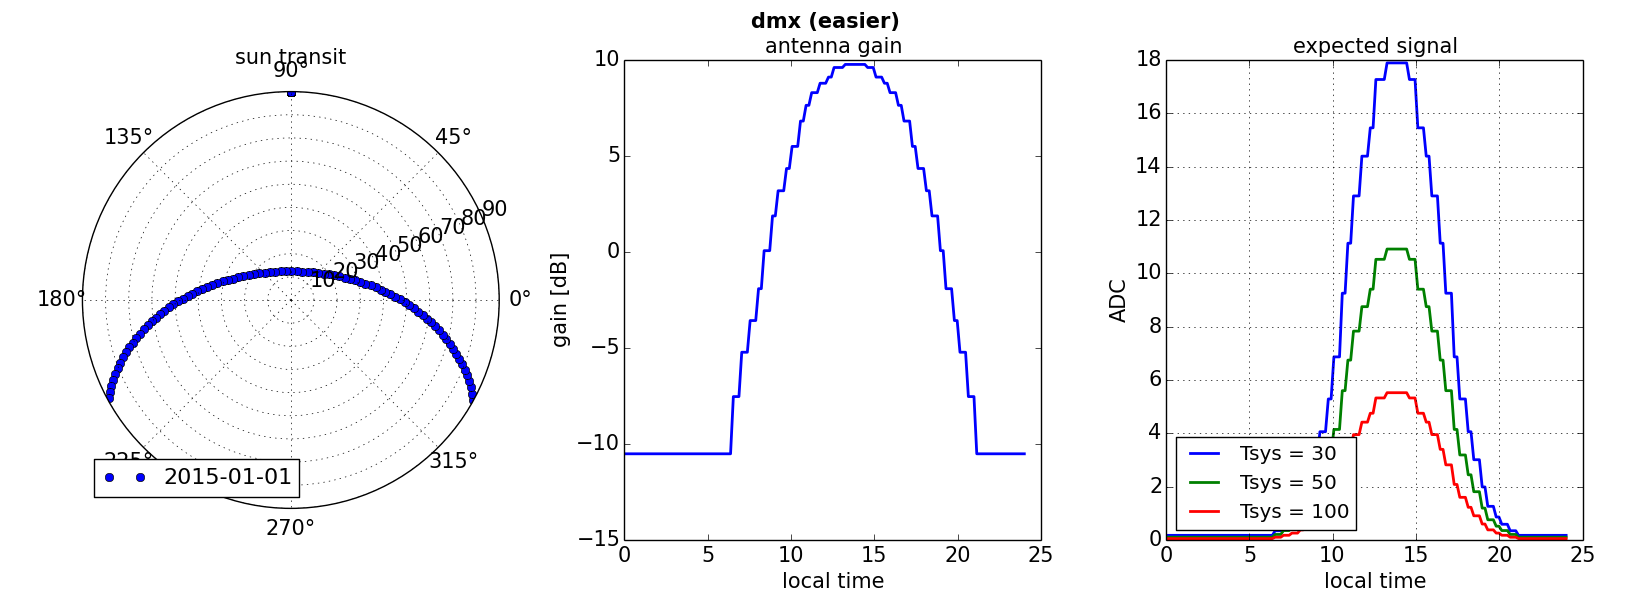
\includegraphics[width=0.7\linewidth]{expeasier.png}}\\
  \subfigure{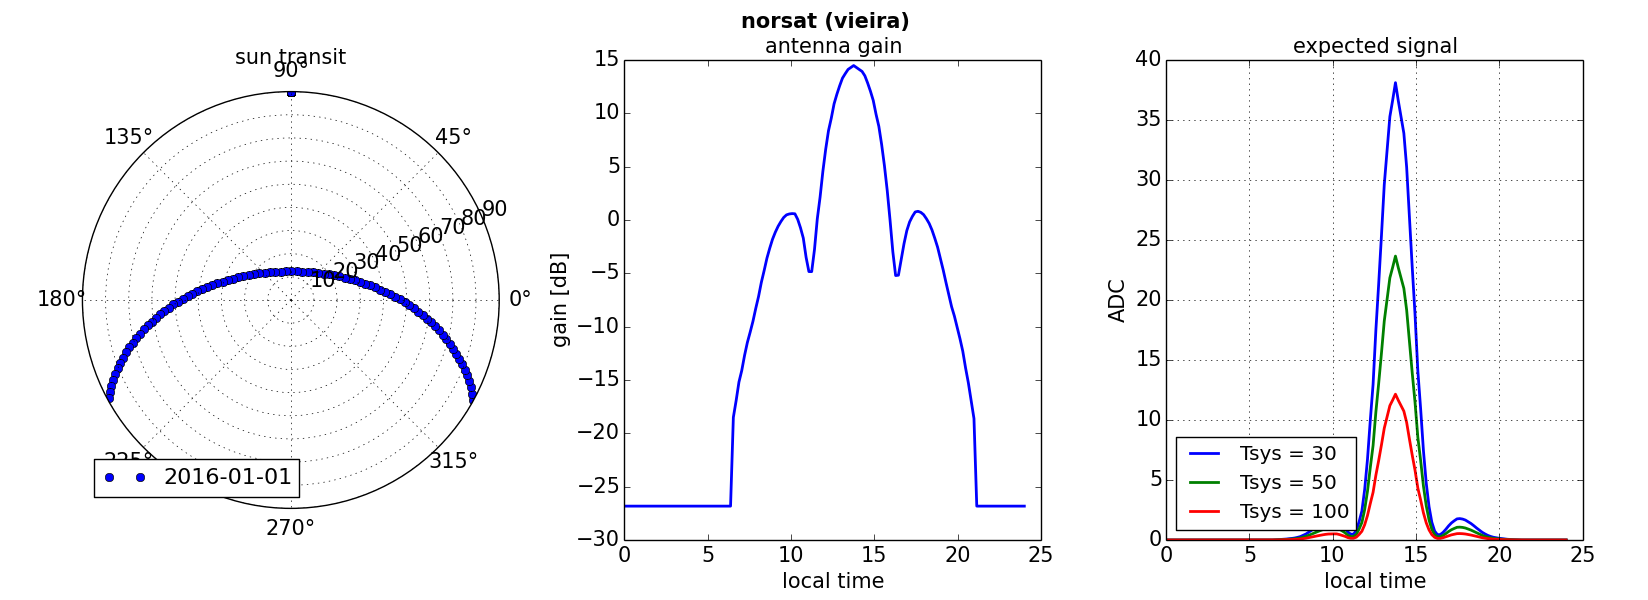
\includegraphics[width=0.7\linewidth]{expvieira20160101.png}}\\
%  \subfigure{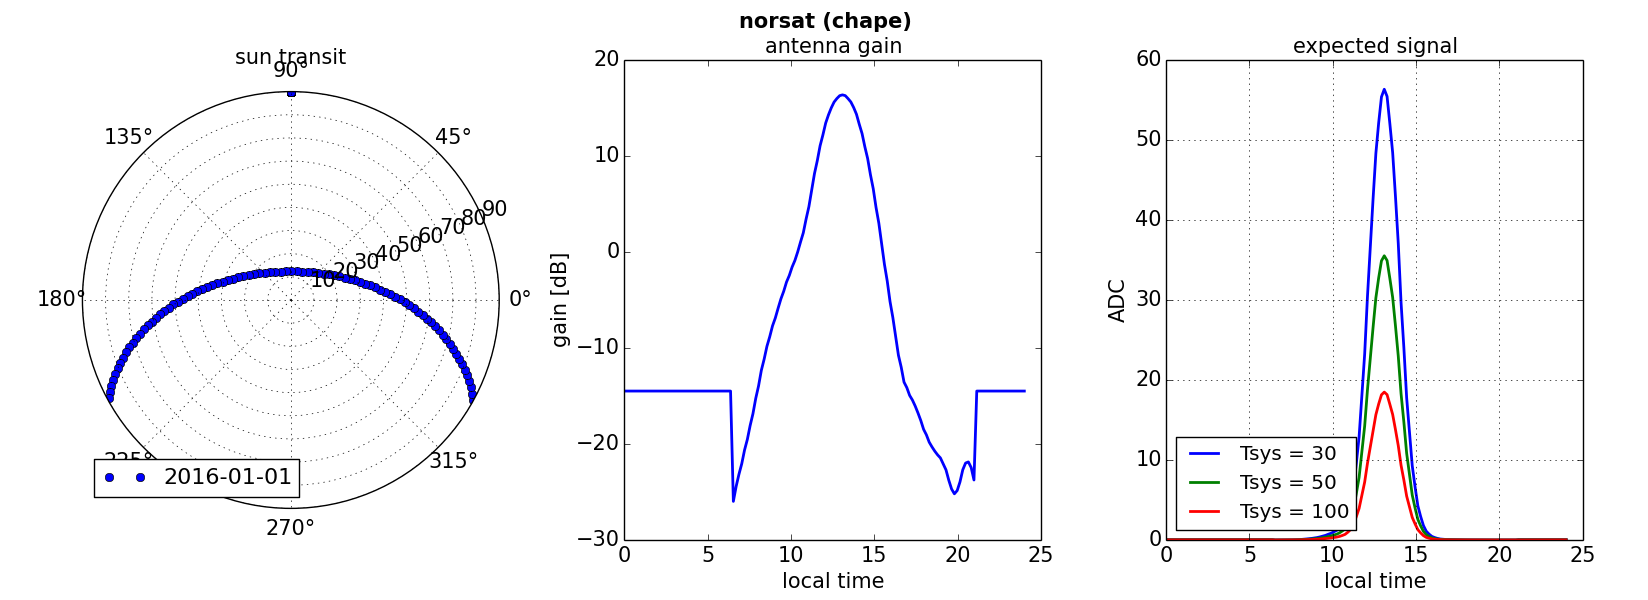
\includegraphics[width=0.7\linewidth]{expchape20160101.png}}\\
%  \subfigure{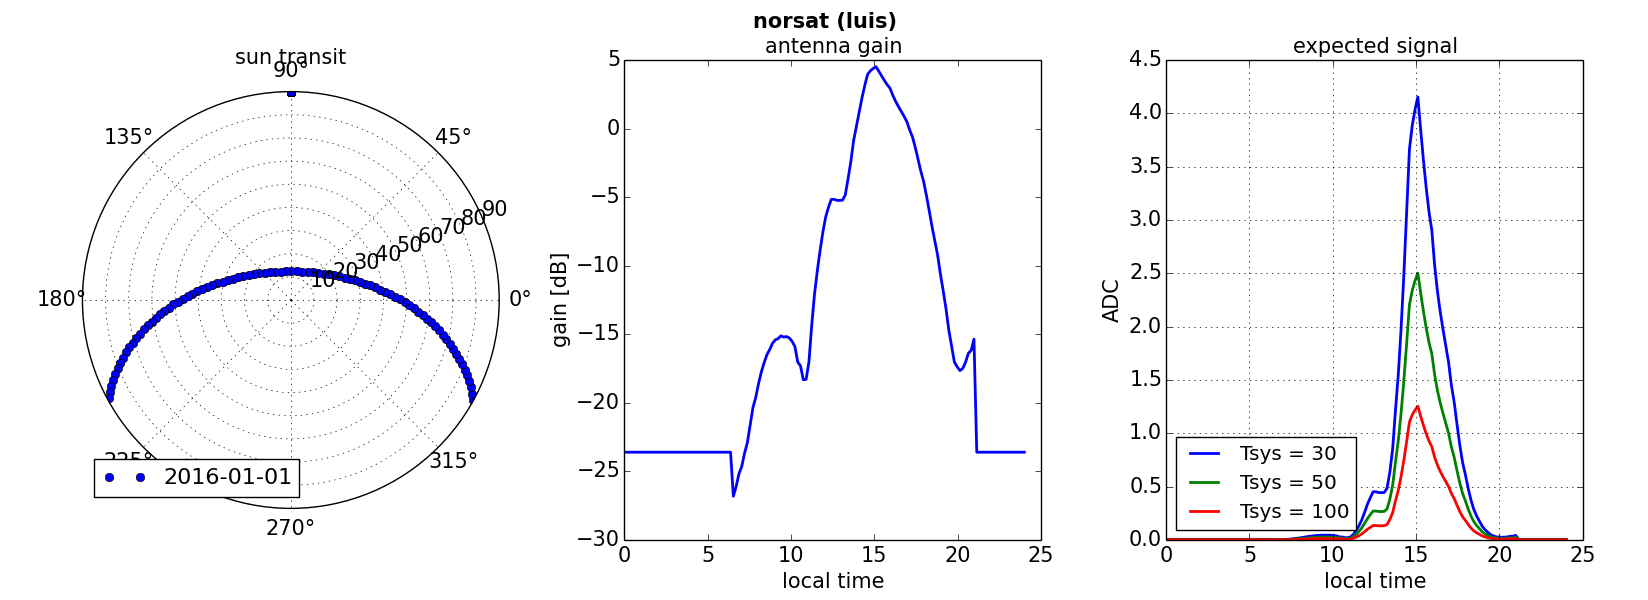
\includegraphics[width=0.7\linewidth]{expluis20160101.png}}\\
  \caption{Expected signal from the  sun for the EASIER detector (top)
    and GIGADuck (bottom). The three pannels indicate the from left to
    right: the  sun path in the  sky, the gain in  the sun's direction
    during  the  day, the  expected  signal  in  ADC count  for  three
    different system temperatures.}
  \label{fig:completesim}
\end{figure}
The expected signal in EASIER is small, and other effects than the sun
can affect the baseline with such  amplitude. We will only use the sun
for the  GIGADuck antennas.  EASIER  detector will be  calibrated with
another method described  in section\ref{sec:easier}.
%% \begin{figure}[!ht]
%%   \centering
%%   \hspace*{-3ex}
%%   \subfigure{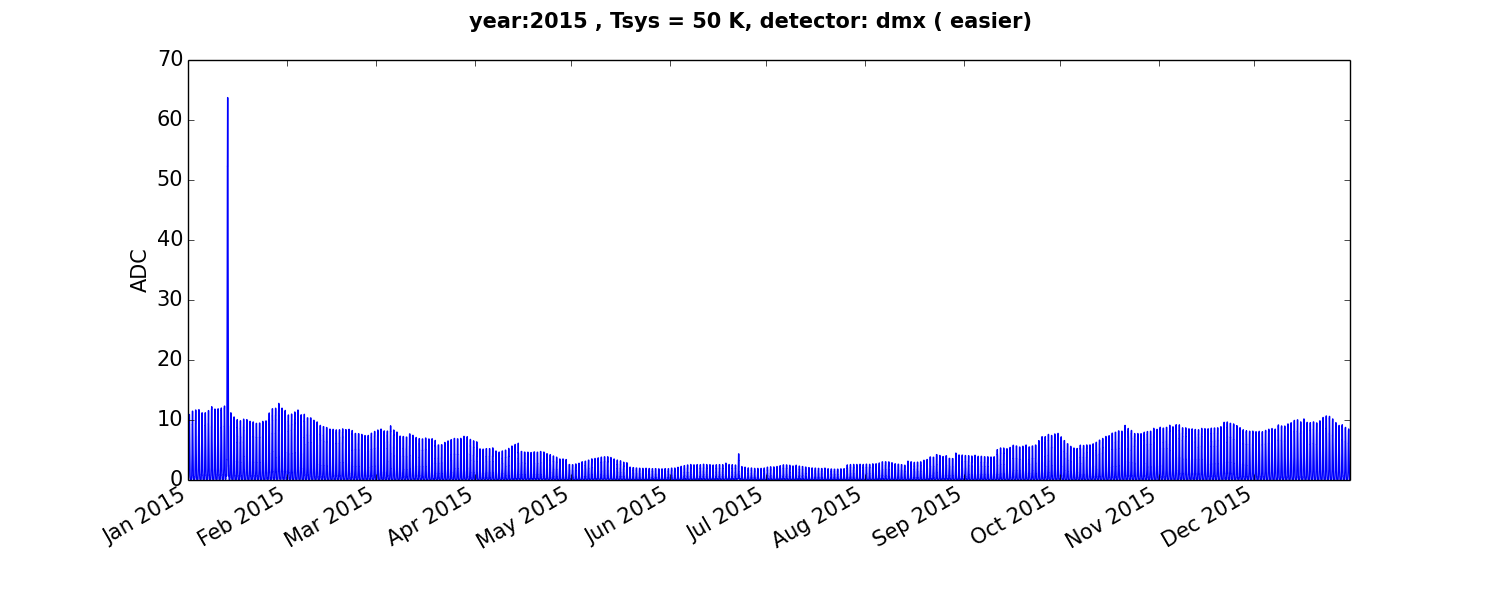
\includegraphics[width=0.7\linewidth]{year2015easier.png}}\\
%%   \subfigure{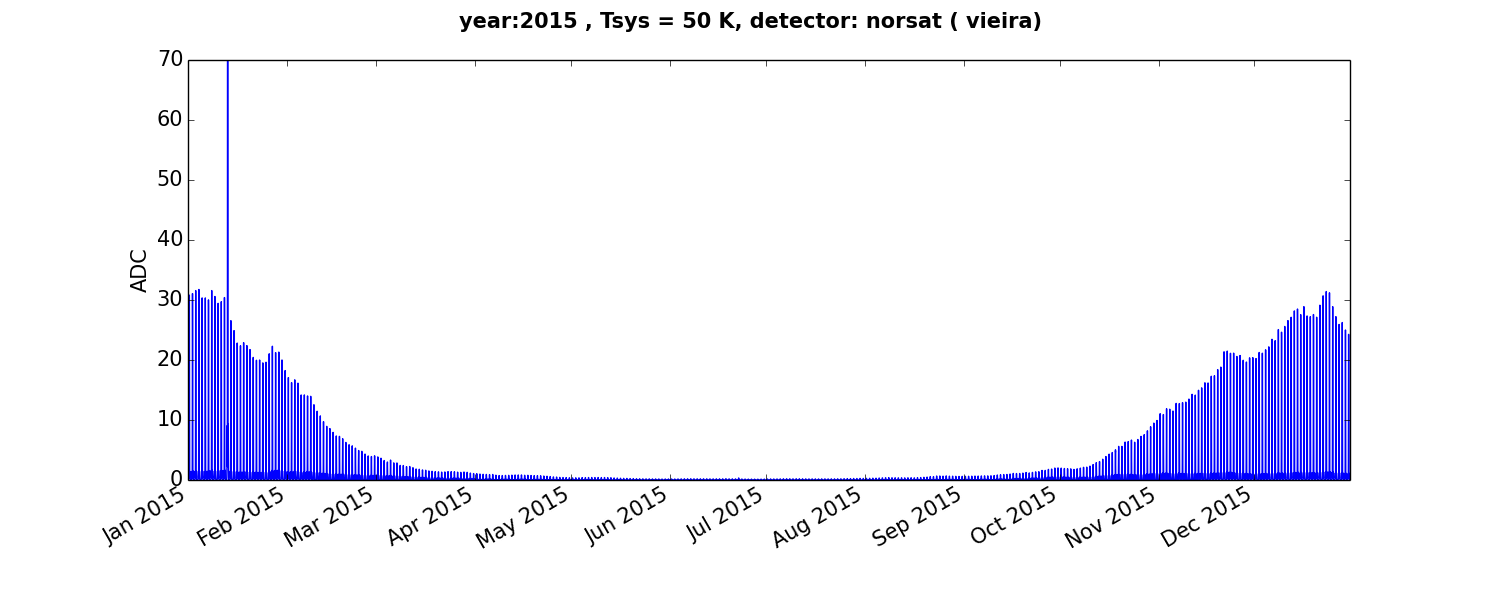
\includegraphics[width=0.7\linewidth]{year2015vieira.png}}\\
%%   \subfigure{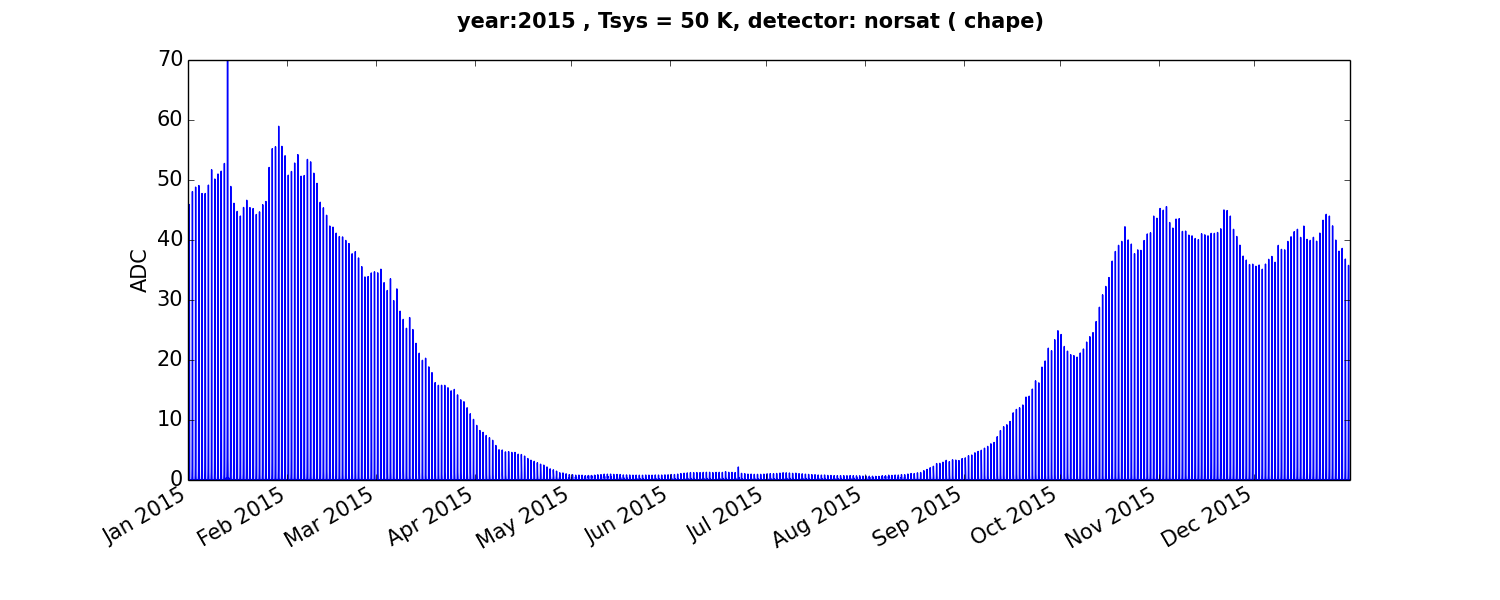
\includegraphics[width=0.7\linewidth]{year2015chape.png}}\\
%%   \subfigure{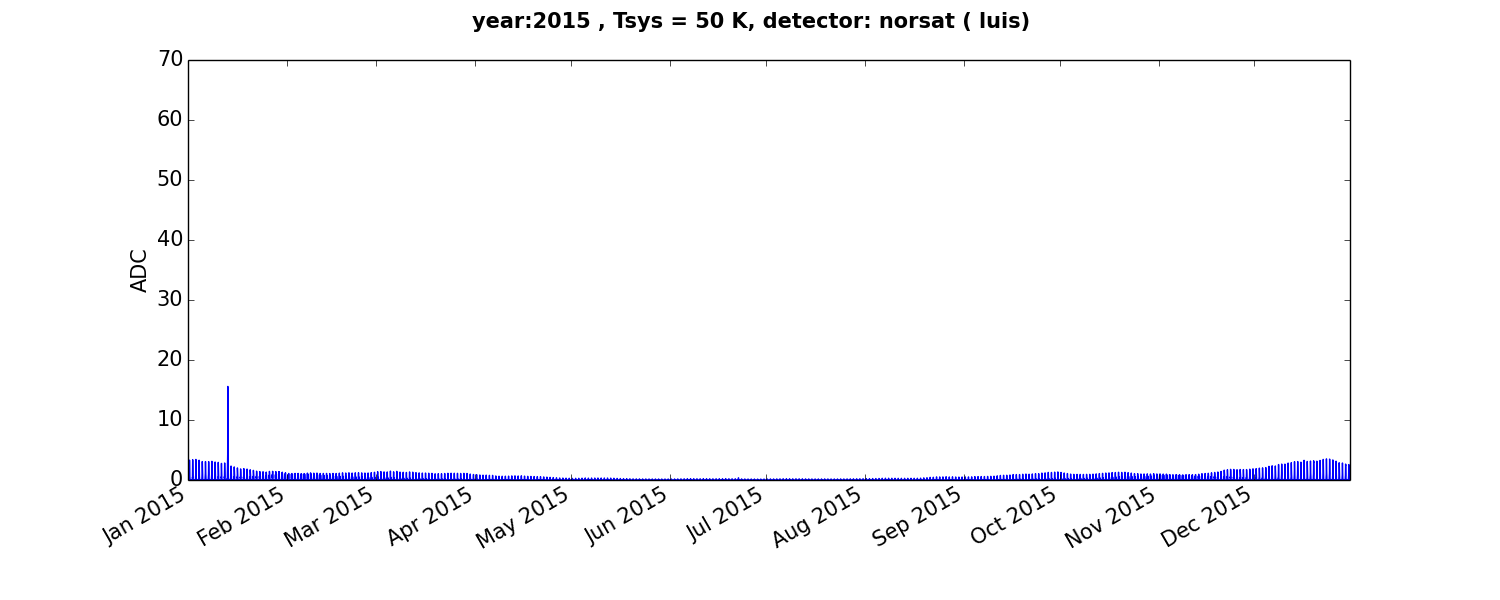
\includegraphics[width=0.7\linewidth]{year2015luis.png}}\\
%%   \caption{Left: quiet sun spectrum, Right: varying component spectrum}
%%   \label{fig:spectra}
%% \end{figure}


